\documentclass[11pt,a4paper]{article}
\usepackage[utf8]{inputenc}

\usepackage{geometry}
 \geometry{
 left=25mm,
 top=25mm,
 right=25mm,
 bottom=25mm,
 }
\usepackage{graphicx}
\usepackage{bm}
\usepackage{url}
\usepackage{amsmath}
\usepackage{tikz}
\usepackage{todonotes}
%\renewcommand{\baselinestretch}{1.25}

\title{Decoding Performance of Convolutional Codes}
\author{Rasmus Vestergaard, Stefan Bejan and Daniel Pytlos}
\date{March 2017}

\begin{document}
\maketitle

\todo[inline] {Compare different codes with the same constraint length but different (same number of) generator polynomials in both burst-error and random-error correction.}

\todo[inline] {Compare different codes with the same constraint length and different code rate (more generator polynomials).}

\section{Decoding Performance in BSC}
The results obtained for the initially given code polynomials are presented in this section. By examining the result for the BSC on figure \ref{fig:givenRandomFigure}, it can be seen that the code with the highest code rate performs best. This is expected, since more redundancy is added. The constraint length does not appear to have a major influence on the performance in this channel, but it is hard to conclude anything when varying multiple parameters at once. Therefore, codes with fixed constraint length are compared in section \ref{sec:constantContraintLengthSection}.
For the burst simulations, it is seen in figure \ref{fig:givenBurstFigure} that Code 1 on average has significantly more errors in the message than the two other codes when comparing at the same burst length.
The result for the MBEC is more interesting. Here, the winner is less clear, and Code 1 and Code 2 perform equally well at low CER, while Code 2 performs best higher values. However, the code rate of Code 1 is only $1/2$ in contrast to the code rate of $1/3$ for Code 2, so it seems that the constraint length do have a big influence in this channel. This is investigated further in section  \ref{sec:constantCodeRateSection}.

\begin{figure}
\centering
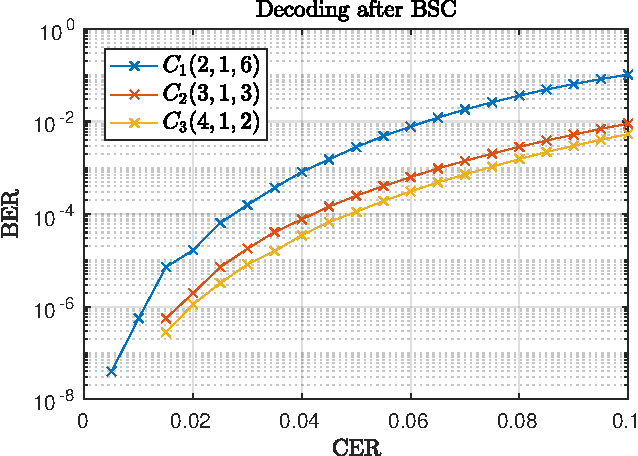
\includegraphics[scale=1]{../figures/qirandom.pdf} 
\caption{\textit{Comparison of given codes in BSC}\label{fig:givenRandomFigure}}
\end{figure}

\begin{figure}
\centering
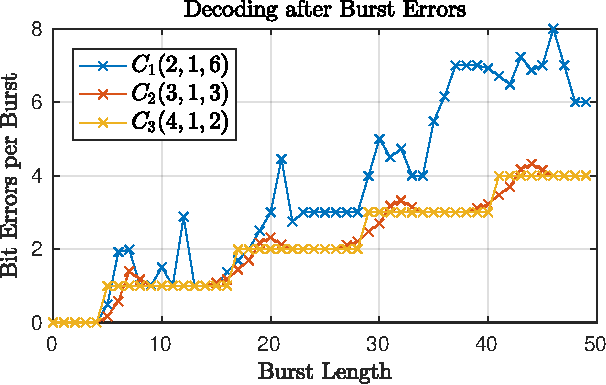
\includegraphics[scale=1]{../figures/qiburst.pdf} 
\caption{\textit{Comparison of given codes burst correction capabilities}\label{fig:givenBurstFigure}}
\end{figure}

\begin{figure}
\centering
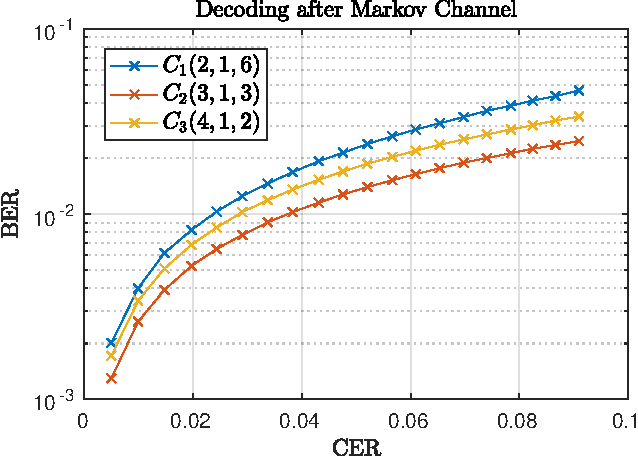
\includegraphics[scale=1]{../figures/qimarkov.pdf} 
\caption{\textit{Comparison of given codes in MBEC}\label{fig:givenMarkovFigure}}
\end{figure}

\section{Decoding Performance with Burst Errors}
This section presents the results obtained by coding the messages with codes having the same code rate (in our case 1/2) but different constraint lengths. Figure \ref{fig:constantCodeRateRandomFigure} indicates that having a higher constraint length reduced the number of decoded errors. However, this is true only for relatively small channel error rates. It can be seen in figure \ref{fig:constantCodeRateRandomFigure} that for our examples, the code with the highest constraint length starts to perform worse than the other at a channel error rate close to 0.08. 
The results of the simulation performed using a channel that introduces bursts errors are shown in figures \ref{fig:constantCodeRateBurstFigure} and \ref{fig:constantCodeRateMarkovFigure}. \todo{Continue here}


\begin{figure}
\centering
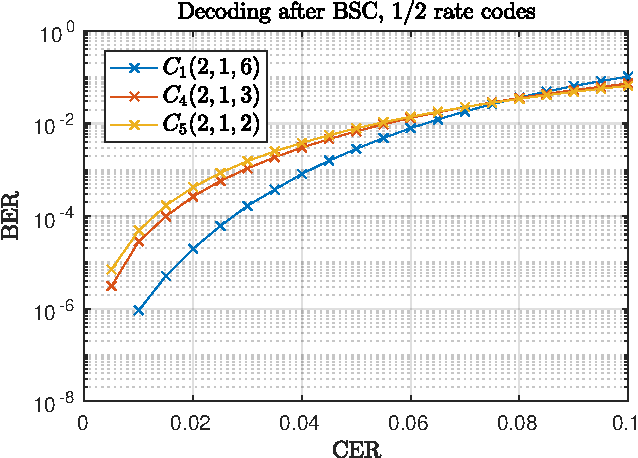
\includegraphics[scale=1]{../figures/extra12rand.pdf} 
\caption{1/2 rate\todo[inline]{change caption}\label{fig:constantCodeRateRandomFigure}}
\end{figure}

\begin{figure}
\centering
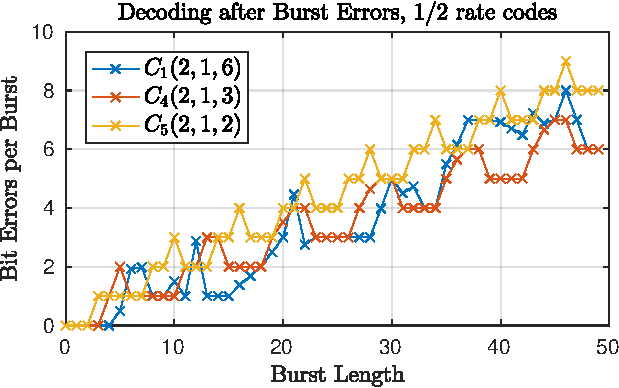
\includegraphics[scale=1]{../figures/extra12burst.pdf} 
\caption{1/2 rate\todo[inline]{change caption}\label{fig:constantCodeRateBurstFigure}}
\end{figure}

\begin{figure}
\centering
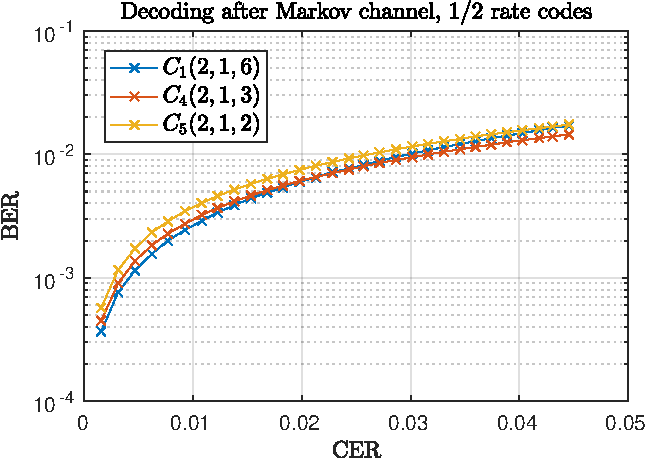
\includegraphics[scale=1]{../figures/extra12markov.pdf} 
\caption{1/2 rate\todo[inline]{change caption}\label{fig:constantCodeRateMarkovFigure}}
\end{figure}
\todo[inline] {Create a markov burst-error channel?}




\end{document}